\chapter{Event reconstruction and simulation}

This chapter overviews the algorithms used to reconstruct the trajectories and identify (ID) types of particles produced in proton-proton collisions in CMS, collectively known as Particle Flow (PF), and how these collisions are simulated. Unless otherwise noted, the material in the first section comes from reference \ref{CMS:2009nxa}.

\section{Particle reconstruction}

The PF algorithms combine information from all of the CMS sub-detectors discussed in the previous chapter to reconstruct the particles produced in the collision event. Since many of the particles produced initially in the collision are unstable, decaying before they have time to interact with the sub-detectors, PF reconstructs the stable particles: electrons, muons, photons, and hadrons. The remaining physics objects of interest, jets, missing energy, taus, etc, can be determined from the information provided by the stable PF-IDed particles. 

\indent The different particles are reconstructed and IDed using information from individual sub-detectors, or combinations of sub-detectors. The direction and momentum of charged particles is measured by the tracker. Electrons are reconstructed using tracks and energy deposits in the ECAL. Muons are reconstructed from a combination of tracker and muon chamber data. Photons are reconstructed from energy deposits in the ECAL. Finally, charged and neutral hadrons are reconstructed from energy deposited primarily in the HCAL, with a contribution from energy deposits in the ECAL. The missing transverse energy, an observable of particular importance to this analysis, used to identify DM that does not interact with the detector material, is the modulus of the sum of transverse momenta of all the PF reconstructed particles. 

\indent The basic pieces of information from the subdetectors used by PF are called elements, and consist of charged-particle tracks, muon tracks, and calorimeter clusters. The tracker provides charged-particle track elements. Since the tracker has the best momentum resolution of the subdetectors, it is of critical importance that the tracking efficiency be nearly 100\%, with as low a fake rate as possible, to reduce an excess in reconstructed energy. These two goals are accomplished using an iterative algorithm: first, tracks are seeded using very tight criteria, yielding a low efficiency, but negligible fake rate, then track seed criteria are loosened and hits that clearly belong to a track are removed, resulting in increasing efficiency. The ECAL and HCAL subsystems (ECAL barrel, HCAL barrel, HCAL endcap, PS first layer, and PS second layer) provide cluster elements. The calorimeter clustering algorithm measures the energy and direction of neutral particles (e.g. photons, neutral hadrons), differentiates energy deposits from neutral and charged hadrons, reconstructs electrons, and contributes to the reconstruction of charged hadrons. The algorithm is summarized as follows: cluster seeds are identified as energy deposit peaks over a given energy, from which topological clusters are grown by appending adjacent cells, and last, topological clusters seed PF clusters. An example is shown in Figure~\ref{fig:pf}, where a simple jet is reconstructed into four clusters, shown as dots. 


\begin{figure}[tbh]
\centering
\begin{subfigure}{0.45\textwidth}
\centering
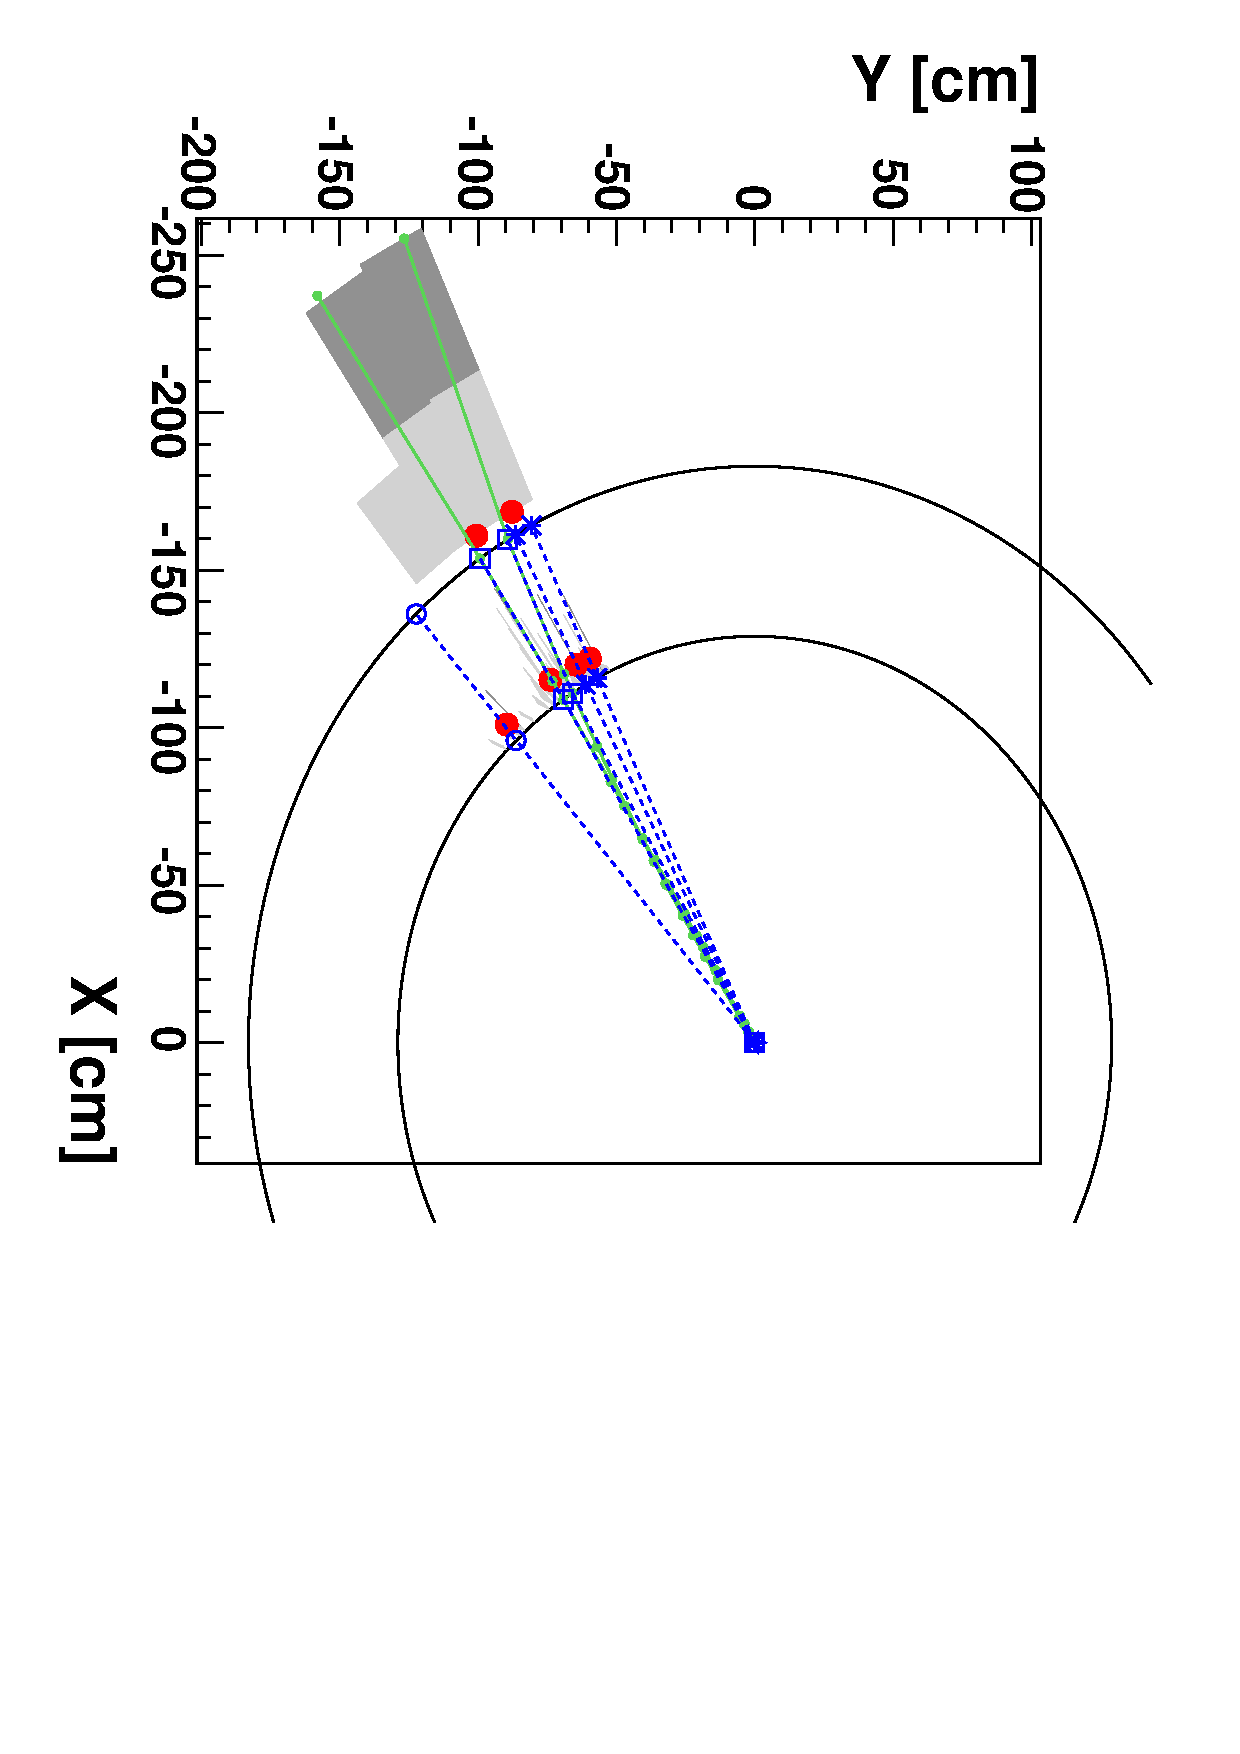
\includegraphics[width=4in]{figures/PFa.pdf}
\caption{}
\end{subfigure}
\begin{subfigure}{0.45\textwidth}
\centering
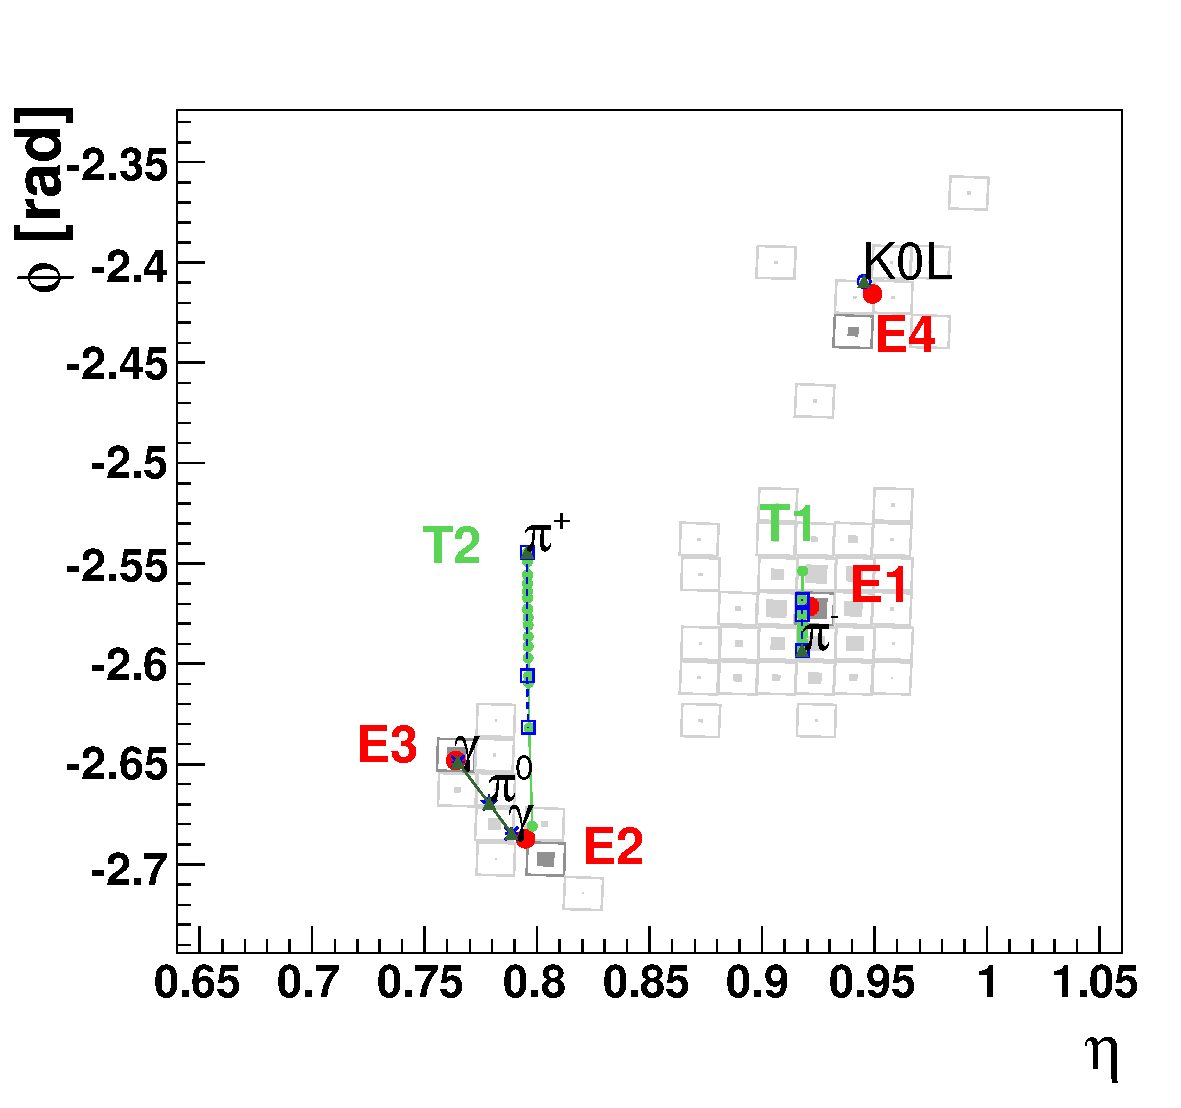
\includegraphics[width=3in]{figures/PFb.pdf}
\caption{}
\end{subfigure}
\begin{subfigure}{0.45\textwidth}
\centering
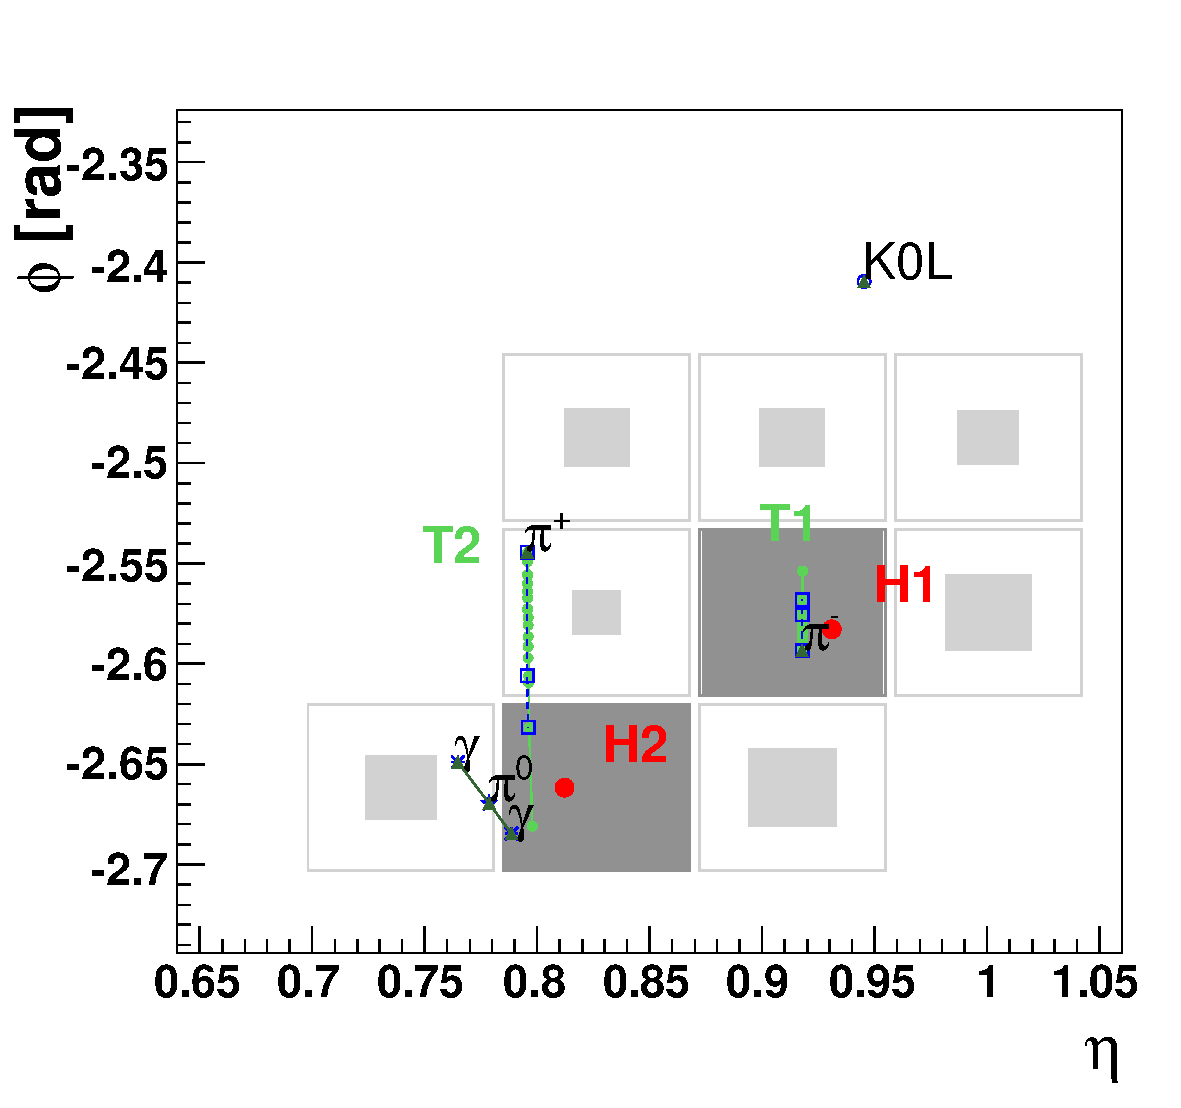
\includegraphics[width=3in]{figures/PFc.pdf}
\caption{}
\end{subfigure}
\caption{Event display of hadronic jet in the x-y plane (a), with solid arcs at the ECAL and HCAL surfaces, and the $\eta-\phi$ plane for the ECAL (b) and HCAL (c). The locations of clusters are given by the solid dots.}
\label{fig:pf}
\end{figure}

\indent Once the PF elements are determined, they are linked together into blocks, which correspond to the signatures left in the sub-detectors of a single particle. Single particles typically leave one to three elements. The linking algorithm determines the quality of the link between all pairwise elements in an event, then forms blocks from the highest quality links, starting from the tracker, and proceeding outward through the calorimeters and muon chambers. Once the blocks are formed, PF associates a global event particle with each block. PF muons are formed from global muon candidates if its momentum is consistent across all track elements. PF electrons are IDed from electron candidates using tracker and ECAL cluster variables, accounting for the Bremsstrahlung photons produced when the electron passes through the tracker material. Once the elements associated to PF muons and PF electrons are removed, the remaining elements are analyzed to ID charged hadrons, photons, or neutral hadrons. PF charged hadrons are associated to remaining tracks if the linked clusters are consistent with the measured momenta. If the energy of the linked clusters is much larger than the track momentum, accounting for uncertainties, a PF photon or PF neutral hadron is formed. Any remaning clusters without linked tracks form PF photons or PF neutral hadrons. 

\indent As previously discussed, once the PF particles are identified, additional information about the event can be inferred. A quantity of particular importance to this analysis is the missing transverse energy (MET), defined above. The performance of the PF algorithms determination of the MET is shown in Figure~\ref{fig:pfmetres} by the resolution of PF measured MET as a function of the true MET to be within $\pm5\%$ above 20 GeV.


\begin{figure}[tbh]
\centering
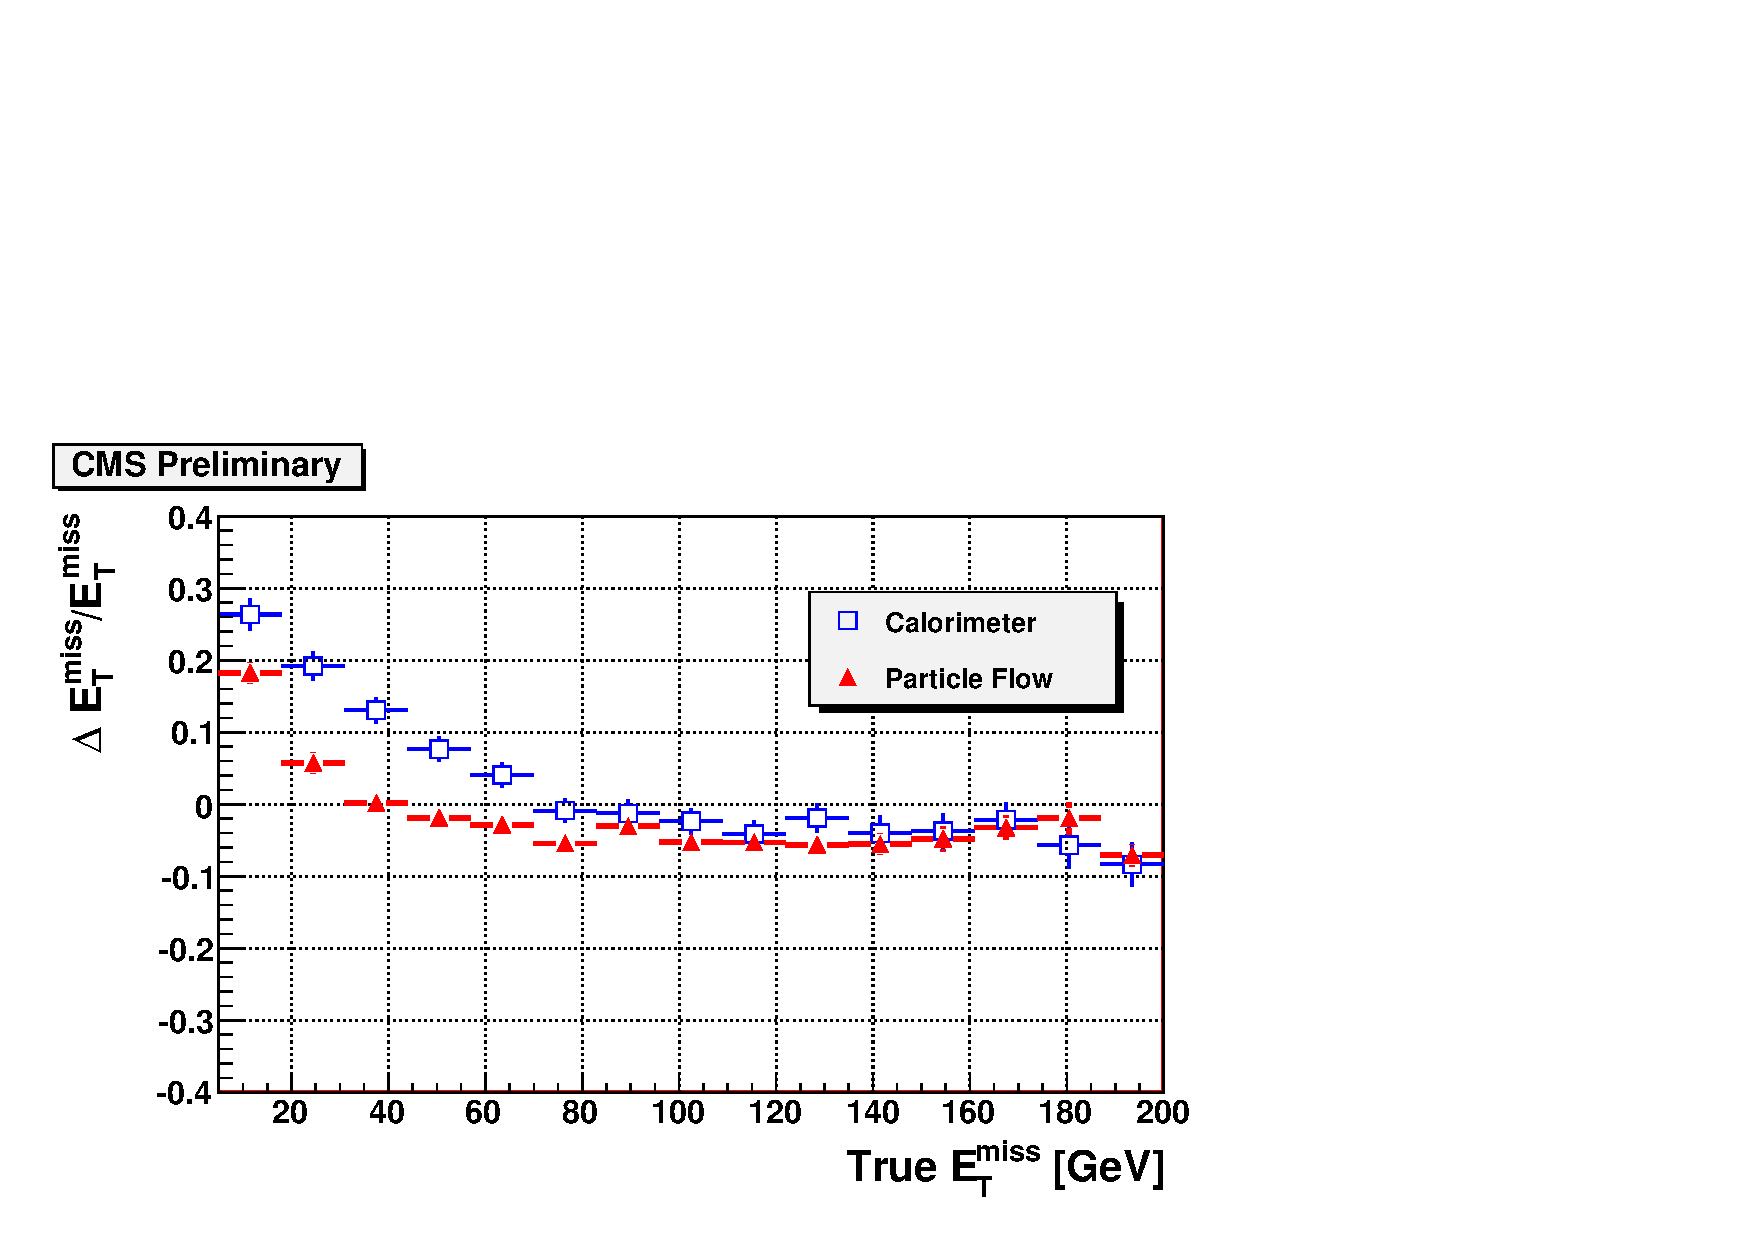
\includegraphics[width=4in]{figures/pfmetres.pdf}
\caption{MET reconstruction resolution.}
\label{fig:pfmetres}
\end{figure}

\section{Monte Carlo event simulation}

The simulation of proton collision events and their detection using Monte Carlo (MC) techniques is useful for several purposes. In addition to using the simulated events to test the detector hardware and software performance without collecting true data, simulations are used to build background models when searching the data for new physics processes. New physics signatures usually appear as excesses in data above a SM background. The background model consists of SM processes which produce the same or similar signature as the new signal being searched for. These processes are modelled either using purely simulated events, or a combination of simulated events and data-driven techniques. In either case, it is often necessary to weight the background events by correction scale factors measured using data, which account for shortcomings of the simulations, such as the inability to perform perturbative QCD calculations for low momentum transfer processes. MC event generation can be factored into two parts: modeling the initial particles produced in a collision event and modeling how these initial particles evolve in and interact with the detector.

\indent The first part of MC event generation is modeling the proton-proton collision and the initial particles produced at the primary vertex. Several software packages are used by CMS analysts to generate collision events and calculate the cross sections of the simulated processes, including PYTHIA \ref{1126-6708-2006-05-026}, MADGRAPH \ref{Alwall2011}, BlackHat and Sherpa \ref{Berger:2009ba}, and POWHEG \ref{Alioli:2010ab}. The packages have different implementations, but the underlying principles are the same. The momenta of the proton partons (quarks and gluons) that interact in the initial scatter are determined probabilistically by random sampling from the parton distribution functions (PDFs), which give the probability that a parton will carry a fraction $x$ of the proton momentum. This is straightforward for processes with two incoming and one outgoing particle ($2 \rightarrow 1$) and two incoming and two outgoing particles ($2 \rightarrow 2$), in which the outcomes are weighted by their relative cross sections and determined probabalistically. For radiative processes such as ISR and FSR of a photon or gluon, generally $1 \rightarrow 2$ processes, higher order matrix elements must be calculated or approximated. Once the initial particles are determined, their fragmentation and decays are simulated in a process called hadronization, until the final stable particles are produced. 

\indent The second part of MC event generation is simulating the detector response to the stable particles produced in the first step, including their interaction with the detector material itself, both active elements and structural material. The primary software package used in this step by CMS is GEANT \ref{documents:998155}, in which a complete digital representation of the CMS detector is built. GEANT simulates the passage of each each stable particle, step-by-step, outward through the detector, probabilistically determining the interaction that occurs at each step depending on the particle's energy,  material it is in, and the EM field present. Since the detector is not perfectly efficienct, both because the acceptance is less than one and the reconstruction efficiency of the individual detector elements is suboptimal, calibration values must be measured at CMS and fed back in to the simulations, so that the performance of the detector can be accurately simulated. Once the final response of the detector is simulated, the resulting MC may be weighted by scale factors measured using real data, in order to correct for mismodelling of the detector.


